%!TEX root = ./template-skripsi.tex
%-------------------------------------------------------------------------------
%                            BAB III
%               		PEMBAHASAN
%-------------------------------------------------------------------------------

\chapter{PEMBAHASAN}

\section{Pengumpulan Data}
\begin{enumerate}
	\item Studi Pustaka\\
	Penulis mendapatkan informasi yang berkaitan dengan steganografi melalui buku referensi dan juga dalam bentuk \emph{e-book}. Penulis juga mencari informasi melalui berbagai situs di internet yang sesuai dengan topik.	
	\item Studi Literatur\\
	Penulis mencoba mencari perbandingan dengan studi sejenis dari beberapa karya ilmiah lokal maupun internasional, seperti jurnal dan skripsi.	 
\end{enumerate}

\section{Perancangan Sistem}

	\subsection{Proses Penyisipan (\emph{Encoding}) pesan ke Citra \emph{Digital}}
	
	\begin{figure}[H]
		\centering
		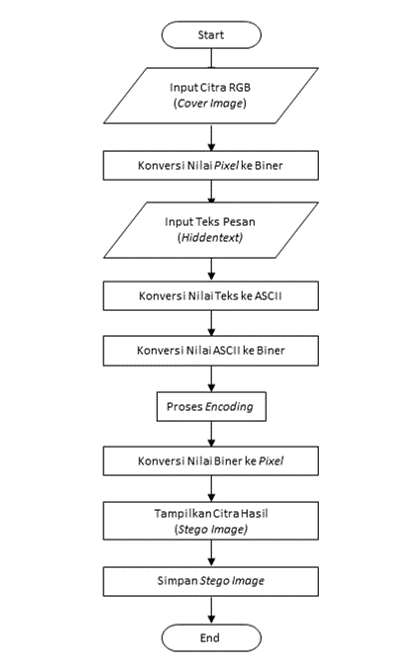
\includegraphics[width=1\textwidth]{gambar/penyisipan3}
		\caption{\emph{Flowchart} Penyisipan Pesan Rahasia}
		\label{flowchart_penyisipan}
	\end{figure}

	Pada gambar di atas adalah \emph{flowchart} proses penyisipan pesan ke dalam \emph{file}
	citra (\emph{Cover Image}). Dimulai dengan membaca \emph{file} citra RGB. Untuk \emph{file} bitmap 24 bit maka setiap \emph{pixel} (titik) pada gambar tersebut terdiri dari susunan
	tiga warna Merah, Hijau dan Biru (RGB) yang masing-masing disusun oleh bilangan 8 bit
	(1 \emph{byte}) dari 0 sampai 255 atau dengan format biner 00000000 sampai 11111111. Setelah
	membaca \emph{pixel} dari \emph{file} citra langkah selanjutnya menentukan bit terkecil (LSB) pada \emph{Cover Image}.
	
	Selanjutnya adalah menyisipkan pesan (\emph{Hiddentext}) yang akan disembunyikan ke dalam \emph{Cover Image}. Pesan tersebut dikonversi terlebih dahulu menjadi nilai ASCII dan kemudian dikonversi kembali menjadi nilai Biner. Setelah itu terjadilah proses penyisipan (\emph{Encoding}). Selanjutnya biner yang telah disisipkan akan dikonversikan kembali ke dalam \emph{pixel}. Dan menyimpan citra yang telah disisipkan pesan ke dalam \emph{Cover Image} sehingga diperoleh atau	dapat ditampilkan sebuah gambar baru (\emph{Stego Image}).
	
	\subsection{Proses Ekstraksi (\emph{Decoding}) pesan dari Citra \emph{Digital}}
	
	\begin{figure}[H]
		\centering
		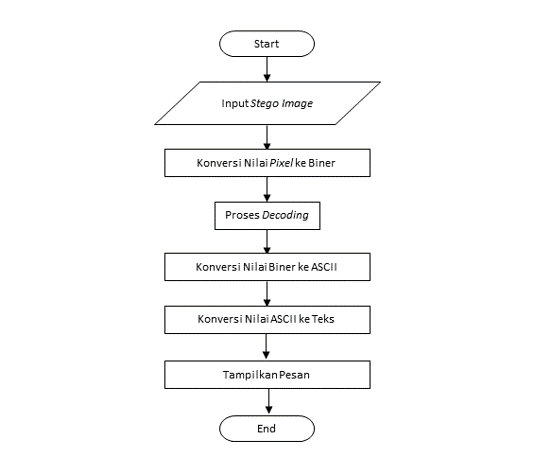
\includegraphics[width=1\textwidth]{gambar/ekstraksi3}
		\caption{\emph{Flowchart} Ekstraksi Pesan Rahasia}
		\label{flowchart_ekstraksi}
	\end{figure}

	Pada gambar di atas adalah \emph{flowchart} proses ekstraksi pesan dari \emph{Stego Image} yang menghasilkan \emph{Hiddentext} yang terdapat di dalamnya. Prosesnya dimulai dengan
	membaca \emph{file} citra, dan mengubah \emph{pixel} ke dalam nilai biner.
	Kemudian proses ekstrasi (\emph{Decoding}). Setelah diperoleh bit-bit yang tersembunyi pada \emph{Cover Image} maka proses
	berikutnya adalah mengkonversi kembali pesan yang tersembunyi (\emph{Hiddentext}), sehingga pesan dapat ditampilkan kembali.

	\subsection{Desain Antar Muka Program}

